% Lecture 22, Fig. 1: in hydrostatic equilibrium the level surfaces of pressure, density and the
% gravity potential coincide; the surface is itself a level surface.
\documentclass[tikz,border=6pt]{standalone}
\usepackage{mathpazo}
\usepackage{bm}
\usetikzlibrary{arrows.meta}
\begin{document}
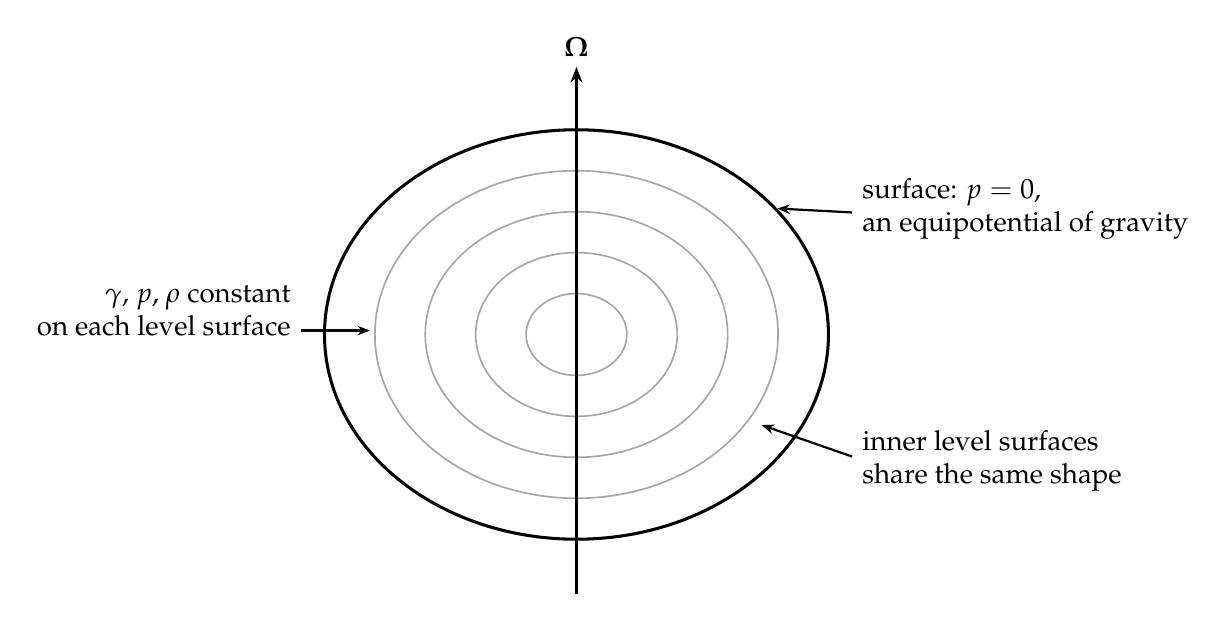
\begin{tikzpicture}[line width=0.8pt]
  \foreach \s/\c in {1.0/black, 0.8/gray!70, 0.6/gray!70, 0.4/gray!70, 0.2/gray!70} {
    \draw[\c, line width={\ifdim \s pt=1pt 1.1pt\else 0.6pt\fi}] (0,0) ellipse ({3.2*\s} and {2.6*\s});
  }
  \draw[-{Stealth[length=2mm]}] (0,-3.3) -- (0,3.4) node[above] {$\bm{\Omega}$};
  \node[align=right, anchor=east] at (-3.5,0.3) {$\gamma$, $p$, $\rho$ constant\\ on each level surface};
  \draw[-{Stealth[length=1.6mm]}] (-3.5,0.05) -- (-2.62,0.05);
  \node[align=left, anchor=west] at (3.5,1.6) {surface: $p=0$,\\ an equipotential of gravity};
  \draw[-{Stealth[length=1.6mm]}] (3.5,1.55) -- (2.55,1.6);
  \node[align=left, anchor=west] at (3.5,-1.6) {inner level surfaces\\ share the same shape};
  \draw[-{Stealth[length=1.6mm]}] (3.5,-1.55) -- (2.35,-1.15);
\end{tikzpicture}
\end{document}
